\section{Target Following in 2D}

We begin with the simplified scenario of following a target in a two-dimensional world.  The following scenario is shown in Figure~\ref{fig:following_2d}.
\begin{figure}[hbt]
  \centering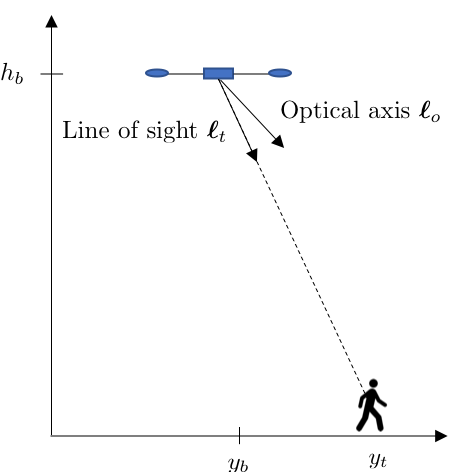
\includegraphics[width=0.5\textwidth]{./figures/following_2d}
  \caption{The following scenario in two dimensions.}
  \label{fig:following_2d}
\end{figure}

We will assume in this section that the body-level dynamics of the camera are given by
\begin{align*}
\ddot{y}_b &= u_1 \\
\ddot{h}_b &= u_2,	
\end{align*}
where the height above ground $h_b$ is in general unknown.  We assume that the optical axis $\boldsymbol{\ell}_o$ is fixed in the body level frame, and that the camera measures 
\[
\boldsymbol{\ell}_t = \frac{\mathbf{p}_{t/\ell}}{\norm{\mathbf{p}_{t/\ell}}}
\]
where
$\mathbf{p}_{t/\ell}= \begin{pmatrix} y_t-y_b, -h_b \end{pmatrix}^\top$.  
The controller also has access to $\dot{\boldsymbol{\ell}}_t$ and $\ddot{\boldsymbol{\ell}}_t$ by numerically differentiating $\boldsymbol{\ell}_t$.  



use "body-level" frame $\mathbf{p}_{\ell/i}$


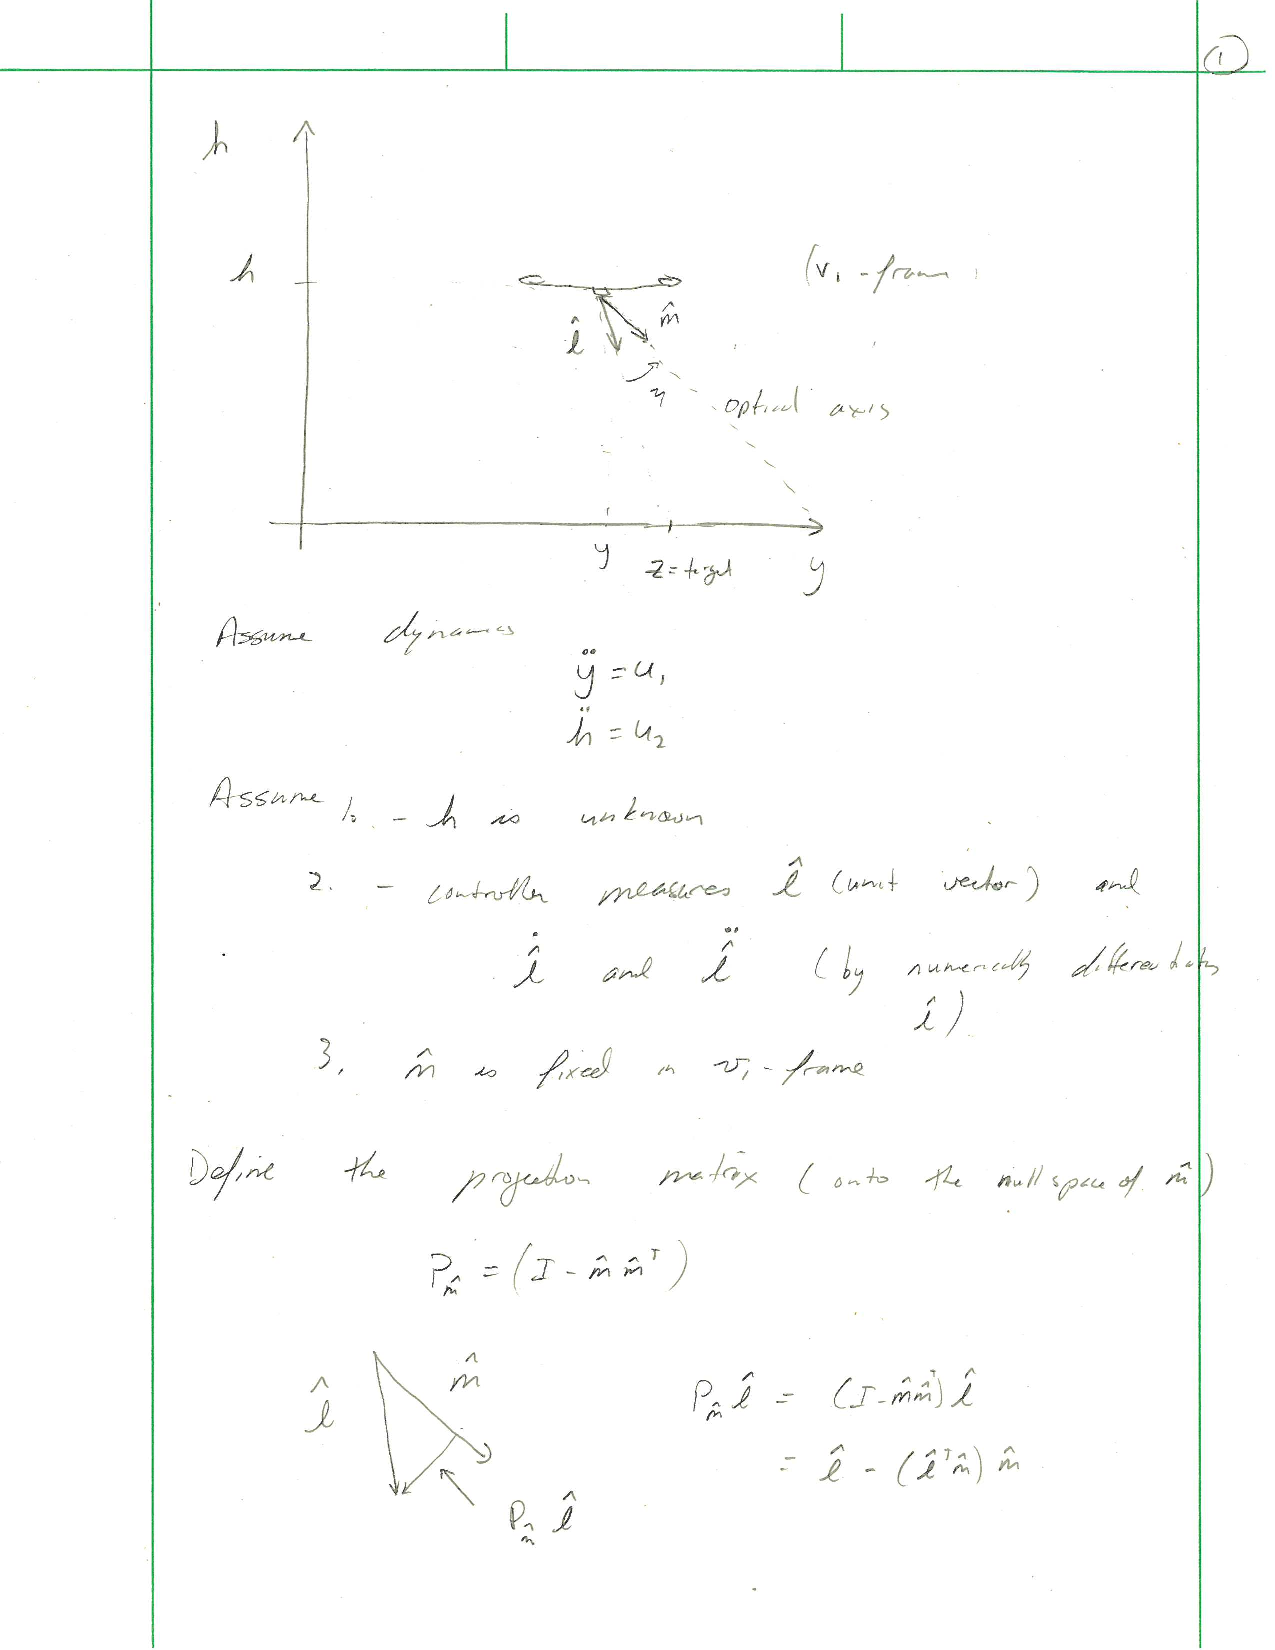
\includepdf[pages=-,scale=.8,pagecommand={}]{adaptive_following_controller.pdf}
